\section{System Operation Chart}
\label{sec:operatingChart}

\todo[inline] {Update Flowcharts and verify whether this text still applies}

Operating charts describe the modes of operation and the flow of the system without much detail. Figure~\ref{fig:systemFlowchart} shows the system's main flowchart, which depicts how the device goes in and out of each of its operating modes.  A general but brief overview of the different modes of operation follows.

\begin{figure}[!ht]
	\centering
	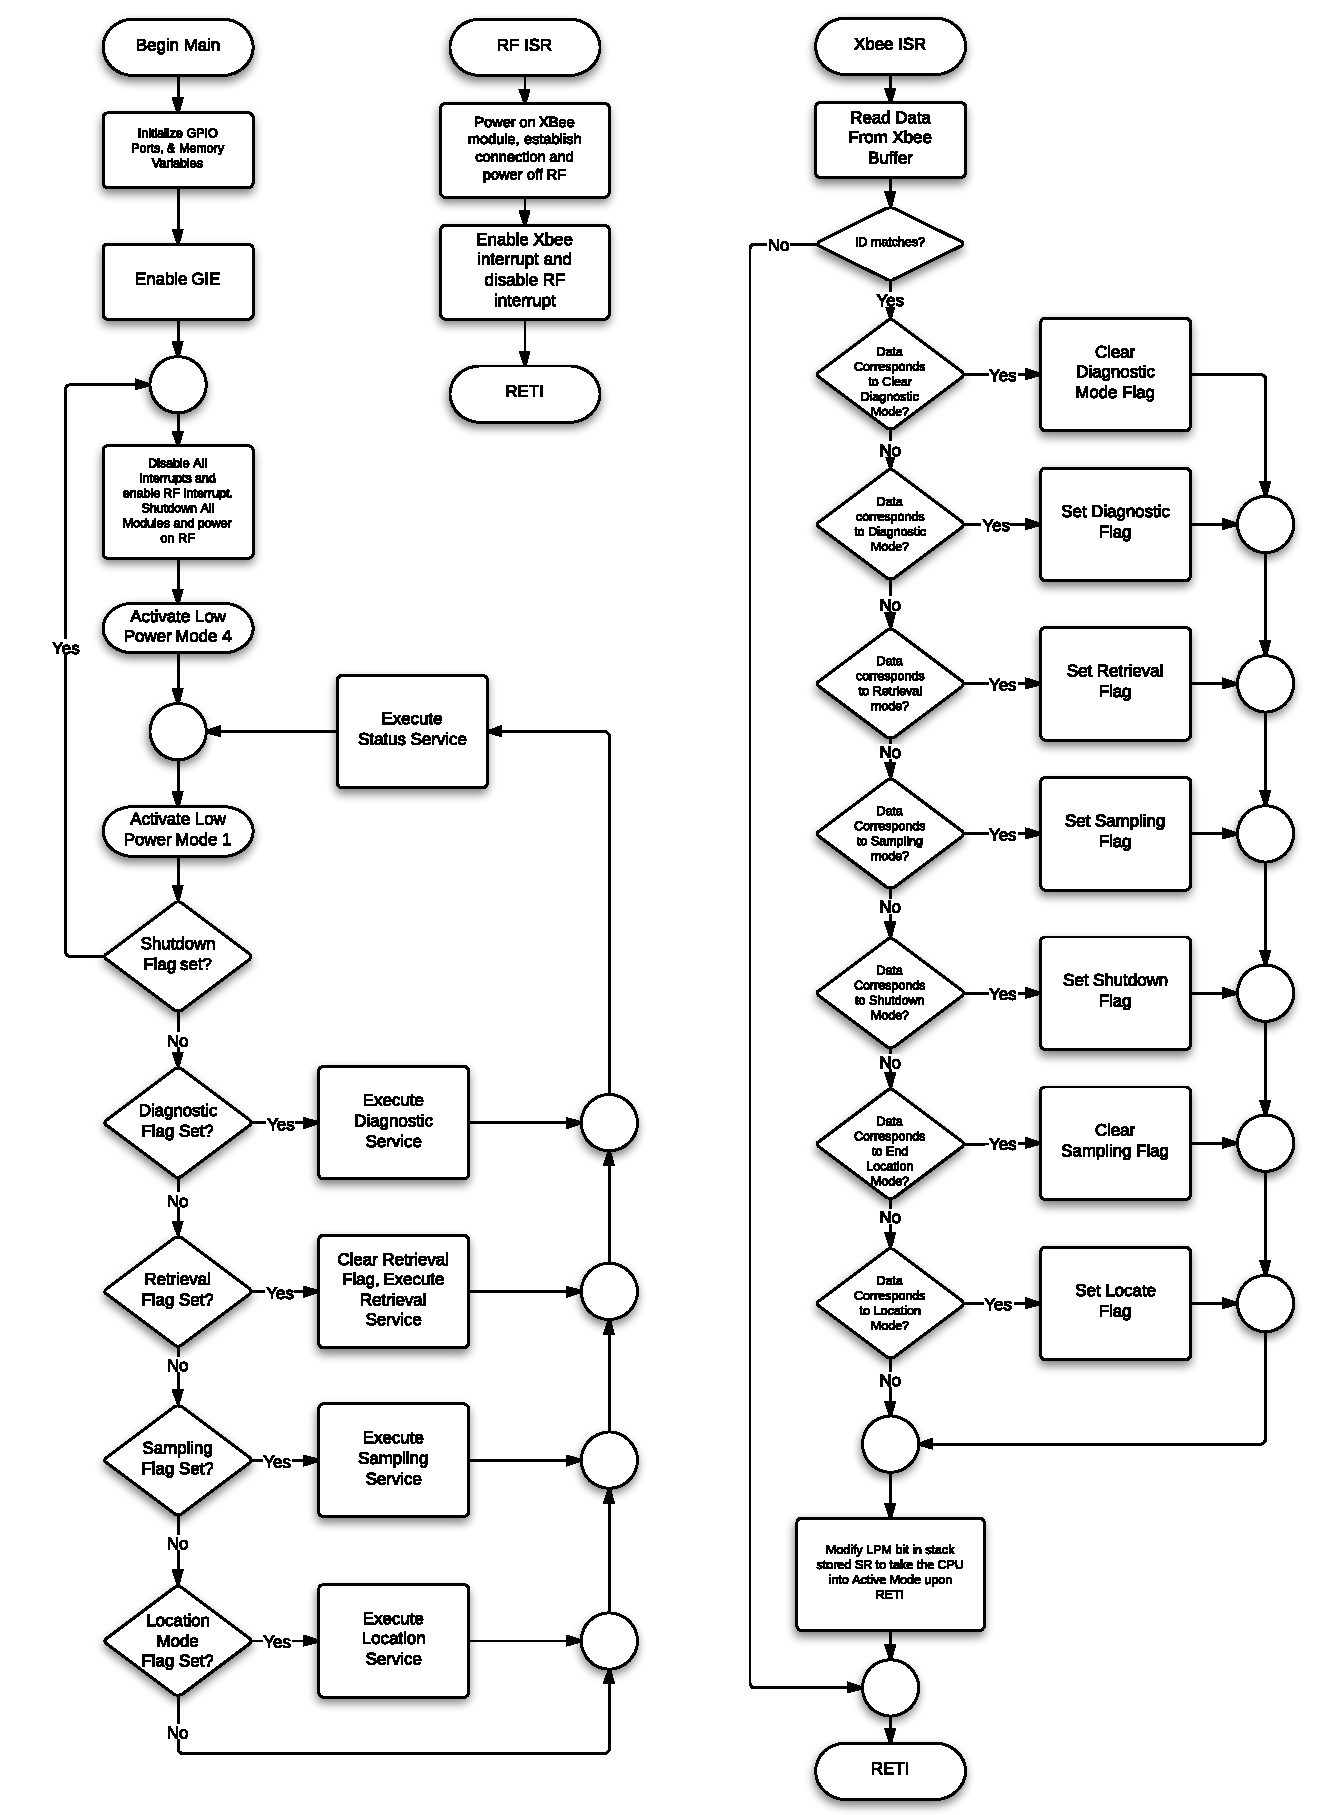
\includegraphics[width=\textwidth]{img/SystemFlowchart}
	\caption{System Main Flowchart. \label{fig:systemFlowchart}}
\end{figure}

When the system is powered up it will perform an initialization sequence, which includes initializing all GPIO ports and memory variables. It will also enable global interrupts and the RF wakeup receiver interrupt while keeping all other interrupts disabled. Subsequently it will power down all other modules except the RF wakeup receiver.

When the initialization sequence is finished, the system will enter a very low power mode. This mode will be called shutdown mode. The system can be woken up by the RF wakeup receiver which will be listening for a specific signal from the user. When the system is interrupted from sleep by the RF wakeup receiver it will power on the XBee module, establish a ZigBee connection, and enable the XBee interrupt. Additionally, the system will power off the RF wakeup receiver and disable its corresponding interrupt.

Afterwards, the system will enter in another low power mode which will be referred to as standby mode. In this mode, the system will maintain an active ZigBee connection via the XBee module. The XBee module will be listening for specific signal from the base station. When it receives a signal, it will interrupt the MCU and set a flag corresponding to the signal that was received. Possible signals are meant for entering diagnostic, retrieval, sampling, status, or shutdown mode. A signal can also be a designation to exit diagnostic mode. The interrupt routine will then take the CPU to active mode, and the system will proceed to execute the service corresponding to the signal that was sent to the XBee module via the base station. After the service has finished executing, the system will return to standby mode where it will listen for more incoming commands.

